
    \subsection{Analisa Paper Rujukan}
	    \label{analisa-paper-rujukan}
		\indent Bercermin terhadap aplikasi \textit{e-commerce} yang telah ada, masalah yang paling sering dialami adalah ketidakpuasan pengguna. Salah satu indikator bahwa suatu perusahaan dikatakan memiliki ketidakpuasan pelanggan adalah karena kegagalan dalam pelayanannya. Seorang pelanggan sangat mungkin memutuskan untuk komplain setelah mengalami ketidakpuasan terhadap layanan suatu perusahaan, dan jika tidak ditangani dengan baik, hal ini bisa berakibat fatal terhadap reputasi dan kepercayaan pengguna terhadap aplikasi tersebut. \\
		\indent Oleh karena itu, sebuah paper mengangkat topik ini khusus dalam bidang aplikasi lelang online, menganalisa kegagalan dan ketidakpuasan pengguna, beserta solusi-solusi yang ditawarkan oleh pengguna aplikasi untuk memperbaiki kegagalan pelayanan tersebut. 
		
	  \begin{figure}[H]
        \centering
        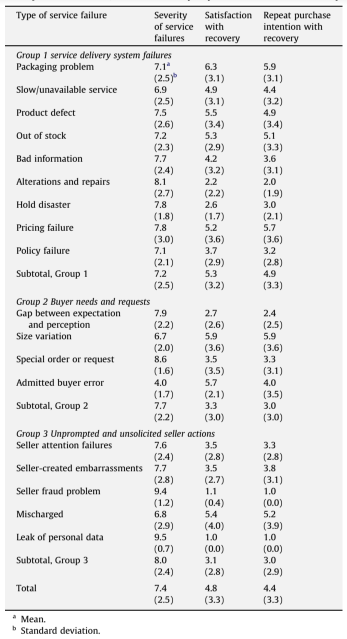
\includegraphics[height=.5\textheight]{images/bab3/Fatalitas-Kegagalan-Ecommerce.png}
        \caption{Fatalitas kegagalan dalam aplikasi Lelang Online, Kepuasan terhadap Perbaikan Pelayanan dan \textit{Repeat Purchase Intention} setelah Perbaikan Layanan}
        \label{severity-failures}
      \end{figure}
      
      \indent Dalam gambar diatas, dijabarkan beberapa jenis kegagalan yang pernah dialami oleh pengguna aplikasi serta fatalitas/pengaruh buruk kegagalan tersebut terhadap kepercayaan pengguna. 
      
	  \begin{figure}[H]
        \centering
        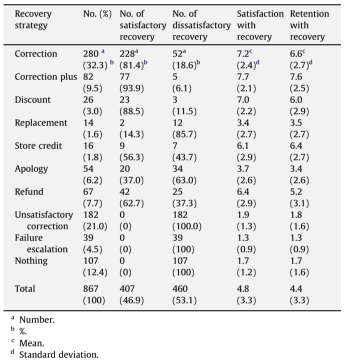
\includegraphics[width=\linewidth]{images/bab3/Solusi-Perbaikan-Ketidakpuasan.png}
        \caption{Kategori Perbaikan terhadap Kegagalan Pelayanan Lelang Online}
        \label{service-recovery-strategies}
      \end{figure}
      
      \indent Maka berdasarkan hasil analisa tersebut, fitur-fitur yang ditambahkan selain daripada fitur dasar aplikasi lelang online sebagai \textit{added vaue} adalah sebagai berikut:
      \begin{enumerate}
      \item Fitur chatting, untuk mengurangi kemungkinan \textit{Bad Information} dimana ekspektasi dan persepsi terhadap barang yang dilelang antara pembeli dan penjual tidak sama dan \textit{Special Needs}, 
      \item Fitur pemberian kupon voucher (\textit{Discount and Correction Plus}) yang bisa berupa \textit{free shipping} atau \textit{discount}.
      \end{enumerate}
  